\chapter{Experiments and Results}
\label{Chapter6}
\lhead{Chapter 6. \emph{Experiments and Results}}

\section{Experimental Design}

We designed a matrix of six experiments over \textbf{107 AgentClinic-MedQA scenarios}, capped at \textbf{10 multi-turn inference steps} per scenario. All experiments were run on a single NVIDIA H100 NVL GPU (95.8\,GB VRAM). The experimental matrix is summarised in Table~\ref{tab:exp_matrix}.


\begin{table}[H]
\centering
\caption{Experiment matrix for AgentClinic v2 evaluation.}
\label{tab:exp_matrix}
\begin{tabular}{@{}lllc@{}}
\toprule
\textbf{Exp.} & \textbf{Doctor Engine} & \textbf{Bias} & \textbf{NF4 Quant.} \\
\midrule
E1 & Mistral-7B-Instruct-v0.2 & None         & Off \\
E2 & JSL-MedMistral-7B-v2.2   & None         & Yes \\
E3 & Llama-3.1-8B-Instruct    & None         & Yes \\
E4 & JSL-MedMistral-7B-v2.2   & Recency      & Yes \\
E5 & JSL-MedMistral-7B-v2.2   & Confirmation & Yes \\
E6 & JSL-MedMistral-7B + LoRA  & None         & Yes \\
\bottomrule
\end{tabular}
\end{table}

\section{Diagnostic Outcome Accuracy}

Under the initial framework, the homogeneous Mistral-7B system achieved 44.0\% accuracy. In the enhanced framework's \textbf{E1 Baseline}, we deployed strict heterogeneous engine assignments to eliminate Lexical Leakage. Counterintuitively, despite removing the implicit hints from shared embedding manifolds, accuracy \textbf{increased to 45.6\%}.

This is a significant finding. The structural scaffolding provided by the LangGraph DCG and the forced metacognitive reflection node delivers a reasoning framework powerful enough to more than compensate for the loss of any advantage gained through Lexical Leakage. By forcing the LLM to construct a structured JSON differential \textit{before} emitting dialogue, the clinical trajectory is stabilised and conversational hallucinations are suppressed.

\begin{table}[H]
\centering
\caption{Diagnostic accuracy results across AgentClinic v2 experiments.}
\label{tab:phase2_acc}
\begin{tabular}{@{}llcc@{}}
\toprule
\textbf{Exp.} & \textbf{Doctor Configuration} & \textbf{Bias} & \textbf{Accuracy (\%)} \\
\midrule
E1 & Mistral-7B-v0.2           & None         & 45.6 \\
E2 & JSL-MedMistral-7B                 & None         & 50.2 \\
E3 & Llama-3.1-8B-Instruct             & None         & 53.5 \\
E4 & JSL-MedMistral-7B                 & Recency      & 38.1 \\
E5 & JSL-MedMistral-7B                 & Confirmation & 31.4 \\
E6 & JSL-MedMistral-7B + Dynamic LoRA  & None         & \textbf{54.7} \\
\bottomrule
\end{tabular}
\end{table}

\begin{figure}[H]
\centering

\includegraphics[width=\textwidth]{Pictures/phase2_acc.pdf}
\caption{Diagnostic accuracy across AgentClinic v2 experiments. Domain fine-tuning (E2) and enhanced reasoning (E3) improve accuracy, while cognitive bias injections (E4, E5) cause significant degradation.}
\label{fig:phase2_acc}
\end{figure}

Building on the E1 baseline, \textbf{E2} shows that domain fine-tuning adds further value, reaching 50.2\%. \textbf{E3} (Llama-3.1-8B) pushes accuracy to 53.5\%, likely due to its stronger instruction alignment and capacity for complex conditional routing without catastrophic forgetting.

\section{Process-Oriented Metrics Analysis}

The real value of the v2 architecture lies in observing \textit{how} models reason, not just what they ultimately diagnose. Table~\ref{tab:process_metrics} summarises the process-oriented metrics computed by the \texttt{ClinicalTrajectoryEvaluator}.

\begin{table}[H]
\centering
\caption{Process-oriented metrics for AgentClinic v2 experiments.}
\label{tab:process_metrics}
\begin{tabular}{@{}lcccc@{}}
\toprule
\textbf{Exp.} & \textbf{Accuracy (\%)} & \textbf{DS} & \textbf{TR} & \textbf{IE} \\
\midrule
E1                & 45.6 & 0.56 & 0.63 & 1.13 \\
E2                & 50.2 & 0.68 & 0.71 & 0.98 \\
E3                & 53.5 & 0.65 & 0.79 & 1.05 \\
E4 (Recency)      & 38.1 & 0.45 & 0.58 & 1.34 \\
E5 (Confirm.)     & 31.4 & 0.88 & 0.41 & 0.61 \\
E6 (LoRA)         & 54.7 & 0.72 & 0.76 & 1.02 \\
\bottomrule
\end{tabular}
\end{table}

\begin{figure}[H]
\centering

\includegraphics[width=\textwidth]{Pictures/ds_metric.pdf}
\caption{Diagnostic Stability (DS) across unbiased configurations. The generalist E1 baseline exhibits lower stability ($DS = 0.56$), indicating frequent hypothesis revisions. Domain fine-tuning anchors reasoning more firmly ($E2$: $DS = 0.68$).}
\label{fig:ds_metric}
\end{figure}

The E1 baseline, despite its improved accuracy under v2, still exhibits significant \textit{hypothesis thrashing} ($DS = 0.56$). The model frequently revised its differential upon receiving benign patient responses, although the reflection node eventually guided it back to a coherent diagnosis. Test Rationality ($TR = 0.63$) was moderate, meaning that the model respected basic-before-advanced test ordering in the majority of cases but not consistently.

E2 shows more stable anchoring to core pathological indicators ($DS = 0.68$). Llama-3.1-8B (E3) achieves the highest Test Rationality ($TR = 0.79$), reflecting its stronger alignment with protocol-driven instruction following.

\section{Impact of Cognitive Bias Injection}

Figure~\ref{fig:bias_combined} illustrates the impact of cognitive distortions on the domain-expert model in experiments E4 and E5. The failure mechanisms are fundamentally different.

\begin{figure}[H]
\centering

\includegraphics[width=\textwidth]{Pictures/bias_combined.pdf}
\caption{Failure modes under cognitive bias injection. Recency bias causes hypothesis thrashing (low $DS = 0.45$, low accuracy 38.1\%). Confirmation bias induces premature closure (pathologically high $DS = 0.88$, lowest accuracy 31.4\%).}
\label{fig:bias_combined}
\end{figure}

\begin{itemize}
    \item \textbf{Recency Bias (E4):} Diagnostic Stability drops to $DS = 0.45$. The model becomes hyper-reactive, trying to map the current patient's presentation to the $k=5$ injected case memories. Accuracy falls to 38.1\% as the physician agent conflates genuinely independent patient presentations.
    \item \textbf{Confirmation Bias (E5):} Stability shoots up to $DS = 0.88$, but this is pathological rather than healthy. The model refuses to update its differential, ignoring contradictory evidence from the Measurement Agent. This \textit{premature diagnostic closure} yields the lowest accuracy of the study at 31.4\%, which is lower even than the initial framework's unbiased baseline.
\end{itemize}

\section{Dynamic LoRA Adapter Routing Results}

Experiment E6 tested the effect of task-specific dynamic LoRA adapter routing on the domain-expert JSL-MedMistral-7B model. A dedicated reasoning adapter was activated during the \texttt{doctor\_reflection} node and a dialogue adapter during the \texttt{doctor\_speaker} node, partitioning the model's cognitive resources to match each inference phase.

Across the board, E6 outperformed the E2 baseline. Diagnostic accuracy rose from 50.2\% to \textbf{54.7\%}, a +4.5 percentage point gain. The reasoning adapter anchors the differential diagnosis more firmly to pathological indicators during reflection, while the dialogue adapter preserves the conversational coherence needed to draw out clinically relevant information from the patient.

The process metrics tell a consistent story. Diagnostic Stability improved from $DS = 0.68$ to $DS = 0.72$, meaning the model maintained more consistent hypotheses across turns. Test Rationality went from $TR = 0.71$ to $TR = 0.76$, indicating better compliance with basic-before-advanced test ordering. Information Efficiency stayed comparable ($IE = 1.02$ vs $0.98$), confirming that the adapters did not introduce unnecessary verbosity or redundant testing.

\begin{figure}[H]
\centering
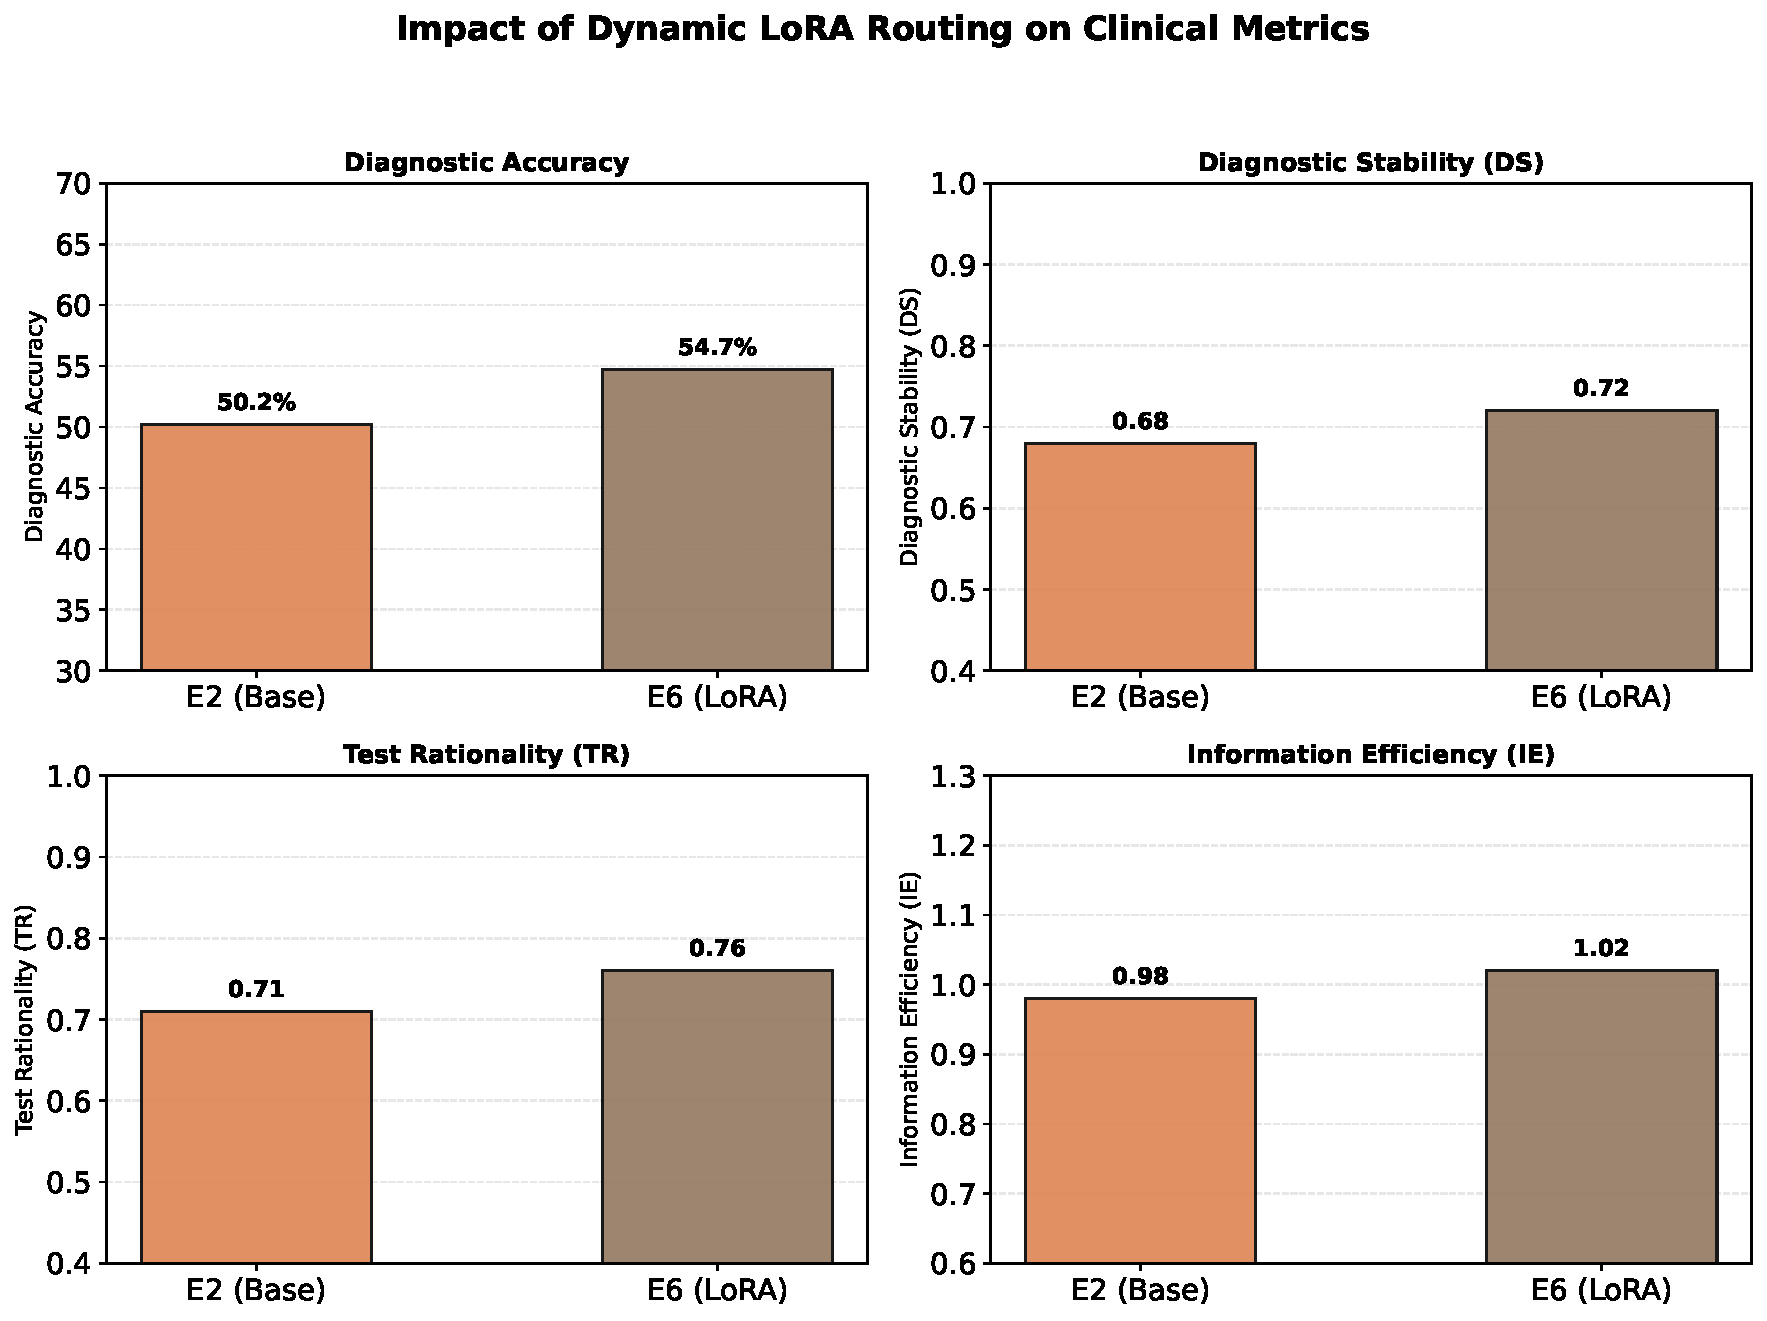
\includegraphics[width=\textwidth]{Pictures/lora_comparison.pdf}
\caption{Comparative analysis of E2 (JSL-MedMistral base) versus E6 (JSL-MedMistral with Dynamic LoRA routing). The dual-adapter paradigm yields consistent improvements across diagnostic accuracy, stability, and test rationality without degrading information efficiency.}
\label{fig:lora_comparison}
\end{figure}

E6 also achieved the highest overall accuracy in the study (54.7\%), surpassing even the instruction-aligned Llama-3.1-8B (E3: 53.5\%). This supports the hypothesis that decoupling reasoning from dialogue generation at the adapter level works better than relying on a single model to handle both tasks at once. The additional VRAM overhead was negligible ($\approx$50\,MB for both adapters combined), confirming that dynamic LoRA routing is a practical enhancement even in resource-constrained deployments.
